\section{Preliminaries}


Henceforth let {\em billiard 3-periodics} refer to the 1d family of Poncelet triangles interscribed between pair of confocal ellipses $\E$ and $\E_c$ given by:
\[ \E:\frac{x^2}{a^2}+\frac{y^2}{b^2}-1=0,\;\;\;\E_c:\frac{x^2}{a_c^2}+\frac{y^2}{b_c^2}-1=0\]
where $c^2=a^2-b^2=a_c^2-b_c^2$.


Billiard N-periodics classically conserve  perimeter $L$ and Joachimsthal's constant $J$. The latter one is equivalent to stating all trajectory segments are tangent to a confocal caustic, see \cite[Thm 4.4]{sergei91} and \cite{arnold2020-joachim}.
When $N=3$, we can derive these explicitly using the vertex parametrization given in \cref{prop:03-vtx-param}.
 

\begin{proposition}
For billiard 3-periodics, the perimeter and Joachimsthal's constant are given by:

\begin{equation*}
J=\frac{\sqrt{2\delta-a^2-b^2}}{c^2},\;\;\;L=2(\delta+a^2+b^2)J
\label{eqn:n3-L-J}
\end{equation*}
where $\delta=\sqrt{a^4-a^2b^2+b^4}$.
\end{proposition}

\begin{proof} We compute the values considering  an isosceles 3-periodic orbit with $P_1=[a,0]$, and

% {\small  
% \begin{equation}\label{eq:isosceles_3orbit}
%  \;  P_2   =\left[-\frac {{a}^{2}\sqrt {2\,\delta-{a}^{2}-{b}^{2}}}{c^2},   
%	\frac { \left(\delta  -{a}^{2}\right) b}{c^2}\right],\;\;
%	    P_3= \left[{-\frac {{a}^{2}\sqrt {2\,\delta-{a}^{2}-{b}^{2} }}{c^2}},
%	{\frac { \left(  {a}^{2}-\delta \right) %b}{c^2}}\right]
%\end{equation}
 %}%
 {\small 
 \begin{equation} \label{eq:orbita3-isosceles}
 P_2=\left[   {\frac {a \left(  {b}^{2}-\delta \right) }{   a^2-b^2 
 			  }},{\frac {{b}^{2}\sqrt {2 \delta -{a}^{2}-{b}^{2}\,
 				}}{{a}^{2}-{b}^{2}}} 
 	\right], \;\; P_3=\left[  {\frac {a \left(  {b}^{2}-\delta \right) }{   a^2-b^2   
 	}},-{\frac {{b}^{2}\sqrt {2\delta-{a}^{2}-{b}^{2} 
 				}}{{a}^{2}-{b}^{2}}} 
 	\right]
 	\end{equation}
 	}
 	We have that
 	\[L=|P_2-P_3|+2|P_1-P_2|,\;\;
 	 J=\langle \frac{P_1-P_3}{|P_1-P_3|},[\frac{1}{a},0]\rangle\]
 	 Straightforward calculations using the vertex parametrization given in \cref{prop:03-vtx-param}, lead to the stated result.
%\textcolor{red}{ronaldo: CAS+parametrization}
\end{proof}

Henceforth the oft-ocurring quantity $\delta$ will be referred to as the Darboux constant. An interesting geometric interpretation for it appears in \cref{prop:03-delta}.

%\noindent Note: the use of $J$ in this chapter refers to its value for the $N=3$ case.

\section{Caustic semi-axes}

The Cayley condition for a concentric, axis parallel (CAP) pair of ellipses to admit a 3-periodic family is given by:

\begin{equation} \frac{a_c}{a}+\frac{b_c}{b}=1
\label{eqn:n3-cayley}
\end{equation}

In turn, this constrains the semi-axes of the confocal caustic.

\begin{proposition}
The semi-axes $a_c,b_c$ of the confocal caustic are given by:
\begin{align*}
a_c=&\frac{a\left(\delta-{b}^{2}\right)}{c^2},\;\;\;\;
b_c=\frac{b\left({a}^{2}-\delta\right)}{c^2}\cdot
\end{align*}
\label{prop:03-n3-caustic}
\end{proposition}

When $a=b$, we have that $a_c=b_c=a/2$.

\begin{proposition}
The semi-axes $a$ and $b$ of the ellipse in terms of the semi-axes $a_c$ and $b_c$ of the confocal ellipse are given by:
\begin{align*}
a&= -\frac{1}{2} \sqrt{w_1} + \frac{1}{2} \sqrt{ w_2 -\frac{ 2 a_c^3 - 4 c^2a_c}{\sqrt{w_1}} } +\frac{a_c}{2},\;\; b=\sqrt{a^2-c^2}\\
w_1&=a_c^2-(4 c a_c b_c)^{\frac{2}{3}},\;\; w_2=2 a_c^2+ (4 c a_c b_c)^{\frac{2}{3}}
\end{align*}
The implicit equation that defines $a$ above is the quartic  given by
\[c^2( a_c^2   - 2   a_c   a )+ a^2(2a_c a  - a^2)=0\]
\label{prop:03-caustic-to-billiard}
\end{proposition}

\section{Incenter and excenter loci}
\label{sec:03-inc-exc-loci}

\begin{figure}
    \centering
    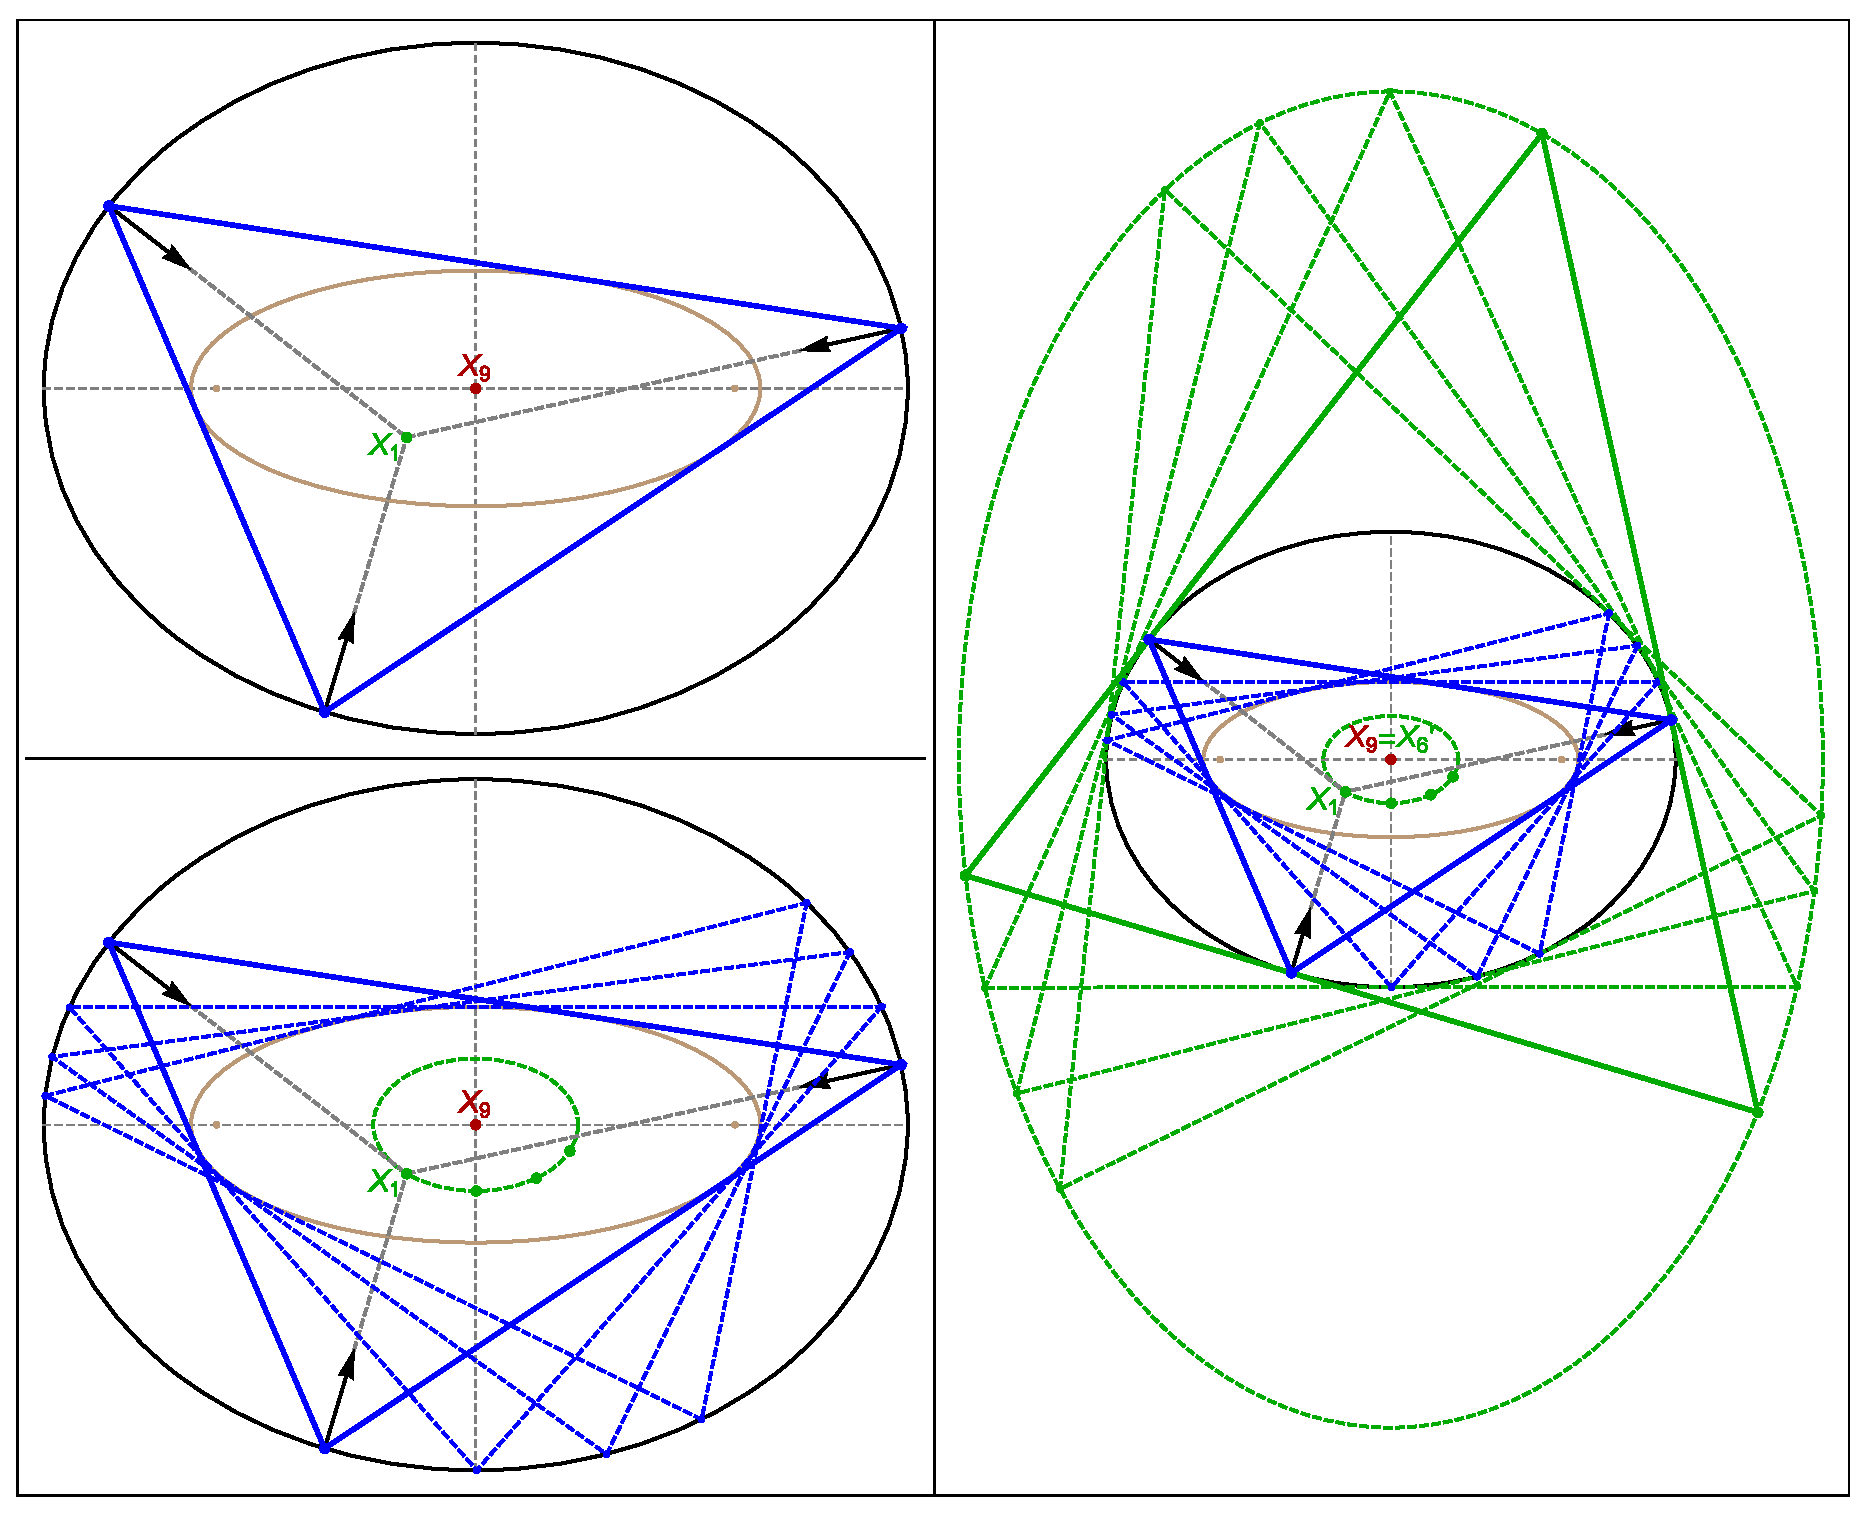
\includegraphics[width=\textwidth]{pics_03_080_billiard_grid.eps}
    \caption{\textbf{Top Left:} An elliptic billiard 3-periodic (solid blue) is shown inscribed in an outer ellipse (black) and a confocal caustic (brown). Graves' theorem implies its internal angles will be bisected by ellipse normals (black arrows). Also shown is the incenter $X_1$ defined as the intersection of said bisectors. \textbf{Bottom Left:} Poncelet's porism implies a 1d family of such triangles exists. Some samples are shown (dashed blue). A classic invariant is  perimeter. The Mittenpunkt $X_9$ remains stationary at the center. The incenter $X_1$ sweeps an ellipse (dashed green). \textbf{Right:} The excentral triangle (solid green) has sides perpendicular to the bisectors. Over billiard 3-periodics, the excentral is of variable perimeter. Its vertices (known as the ``excenters'') also sweep an ellipse (dashed green) whose aspect ratio is the reciprocal of that of the incenter locus. The Symmedian point $X_6'$ of the excentral triangle coincides with $X_9$ of the reference and is therefore stationary. \href{https://bit.ly/3gWl3CI}{Live}}
    \label{fig:billiard-grid}
\end{figure}

An intriguing phenomenon is that over billiard 3-periodics, the locus of both incenter and the excenters are ellipses, as was initially detected experimentally (see an early \href{https://youtu.be/BBsyM7RnswA}{Video}). This was proved by \cite{olga14} and \cite{garcia2019-incenter}. Indeed, we haven't yet found another Poncelet pair where this is the case, see \cref{conj:04-incenter-excenter-loci}.

Referring to \cref{fig:billiard-grid}:

\begin{theorem}
Over billiard 3-periodics, the locus of the incenter $X_1$ and excenter are ellipses $\E_1$ and $\E_e$ concentric and axis-parallel with the confocal pair whose axes $(a_1,b_1)$ and $(a_e,b_e)$ are given by:
\begin{align*}
a_1 =& \frac{\delta-b^2 }{a},\;\;\;b_1=\frac{a^2-\delta}{b}\\ 
a_e= &\frac{{b}^{2}+\delta}{a},\;\;\;b_e=\frac{{a}^{2}+\delta}{b}
\end{align*}
Furthermore, $\E_1$ and $\E_e$ have reciprocal aspect ratios, i.e., $a_1/b_1=b_e/a_e$.
\label{thm:03-incenter-excenter}
\end{theorem}

\begin{proof}
It follows from the vertex parametrization in \cref{prop:03-vtx-param} and the definition of incenter and excenters.  
We have that
\[X_1=\frac{s_1 P_1+s_2P_2+s_3P_3}{s_1+s_2+s_3}=
\frac{1}{L}(s_1P_1+s_2P_2+s_3P_3)\]
where $s_1=|P_2-P_3|$, $s_2=|P_1-P_3|$ and $s_3=|P_1-P_2|$.
A careful symbolic analysis shows that $\mathcal{E}_1(X_1)=0$. A similar analysis considering the excenters shows that the locus of the three points is the ellipse $\mathcal{E}_e$ stated.
\end{proof}

\noindent A more general treatment to the above is given in \cref{chap:04-n3-loci}.

\begin{corollary}
The pair $\{\mathcal{E},\mathcal{E}_e\}$ is Ponceletian.
\label{cor:03-excentral-billiard-poncelet}
\end{corollary}

\begin{proof}
Direct from Cayley condition
\[\frac{a}{a_e}+\frac{b}{b_e}=\frac{a^2}{b^2+\delta}+\frac{b^2}{a^2+\delta}= 1\]

\end{proof}

\section{A stationary point}
\label{sec:03-stationary}

The Mittenpunkt $X_9$ is a triangle center where lines from each excenter thru the side midpoint meet. Referring to \cref{fig:03-x9}:
\begin{theorem}
Over the family of 3-periodics in the elliptic billiard, $X_9$ is stationary at the common center.
\end{theorem}

An elegant syntethic proof was kindly contributed by \cite{olga19_mitten}:

\begin{proof}
Let $\E$ be the outer ellipse in the confocal pair, $O$. By definition, the Mittenpunkt $X_9$ is where lines from the excenters $E_i$ through the side midpoints $M_i$ concur. Notice each side is an ellipse chord between tangents to $\E$ seen from the $E_i$ (this is because in the confocal pair the excentral triangle is tangent to $\E$). Consider the image of lines $E_i M_i$ under an affine transform which sends $\E$ to a circle $\Cm'$, let $O'$ be its center. The transformed lines will pass through the midpoints of chords of $\Cm'$ between tangents seen from $E_i'$ (the affine image of $E_i$). By circular symmetry, such lines must also pass through $O'$, and therefore remain stationary. But $O'$ is the affine image of $O$, so the result follows.
\end{proof}

\begin{figure}
     \centering
    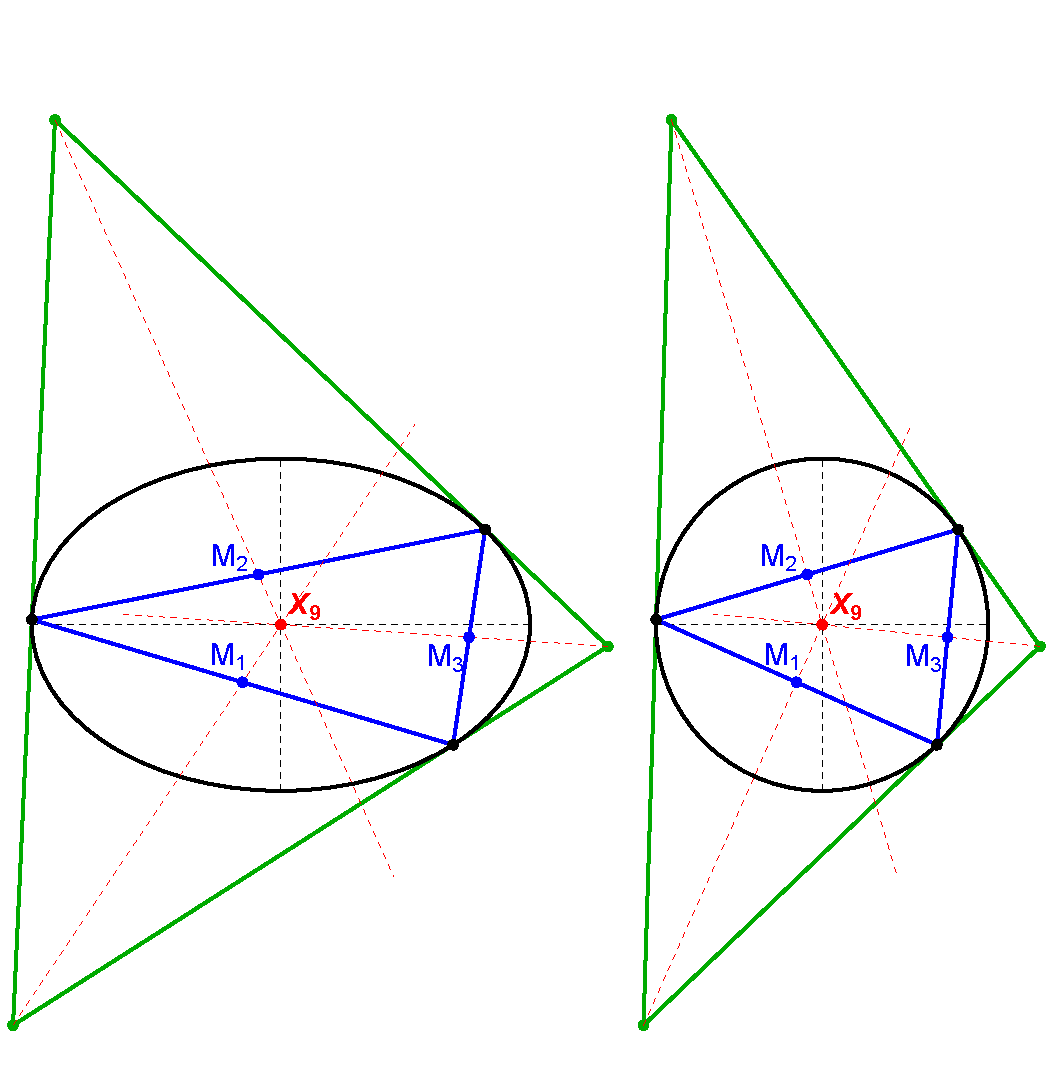
\includegraphics[width=\linewidth]{pics_03_090_mitten_proof.pdf}
     \caption{\textbf{Left}: 3-periodic billiard triangle (blue), its excentral triangle (green). The Mittenpunkt $X_9$ is the point of concurrence of lines drawn from the excenters through sides' midpoints $M_i$. \textbf{Right}: the affine image which sends the billiard to a circle. Lines from imaged excenters through sides' midpoints must pass through the origin. Since the latter is stationary, so must be its pre-image $X_9$, which is stationary at the billiard center.  % done
     \href{https://youtu.be/tMrBqfRBYik}{Video}}
     \label{fig:03-x9} 
\end{figure}

\section{Conserved Quantities}

Given a triangle, let $r$ and $R$ denote the radius of its incircle and circumcircle, known as the {\em inradius} and {\em circumradius}, respectively. Over billiard 3-periodics, note these two radii are variable. Referring to \cref{fig:radii}:

\begin{theorem}
$r/R$ is invariant over the 3-periodic orbit family and given by:
\begin{equation*}
\label{eqn:rovR}
\frac{r}{R}=\frac{2 (\delta-b^2)(a^2-\delta)}{c^4}.
\end{equation*}
\label{thm:03-confocal-rovR}
\end{theorem}

\begin{proof}
The following relation, found in \cite{johnson1960}, holds for any triangle:

\begin{equation*}
 r R=\frac{s_1s_2s_3}{2 L}, 
\end{equation*}

\noindent where $L=s_1+s_2+s_3$ is the perimeter, constant for 3-periodic orbits. Therefore:

\begin{equation}
\frac{r}{R}=\frac{1}{2L} \frac{s_1s_2s_3}{R^2}\cdot
\label{eqn:rovR-cas}
\end{equation}

Next, let $P_1=(a,0)$ be a vertex of an isosceles 3-periodic. Obtain a candidate expression for $r/R$. This yields \eqref{eqn:rovR} exactly. Using the vertex parametrization in \cref{prop:03-vtx-param}, derive an expression for the square of the right-hand side of \eqref{eqn:rovR-cas} as a function of $x_1$ and subtract from it the square of \eqref{eqn:rovR}. In  \cite{garcia2020-new-properties}
it is shown $\left(s_1s_2s_3/R^2\right)^2$ is rational on $x_1$. For simplification, use $R=s_1 s_2 s_3/(4A)$, where $A$ is the triangle area. With a CAS, show said difference is identically zero for all $x_1\in(-a,a)$.
\end{proof}


\begin{figure}
    \centering
    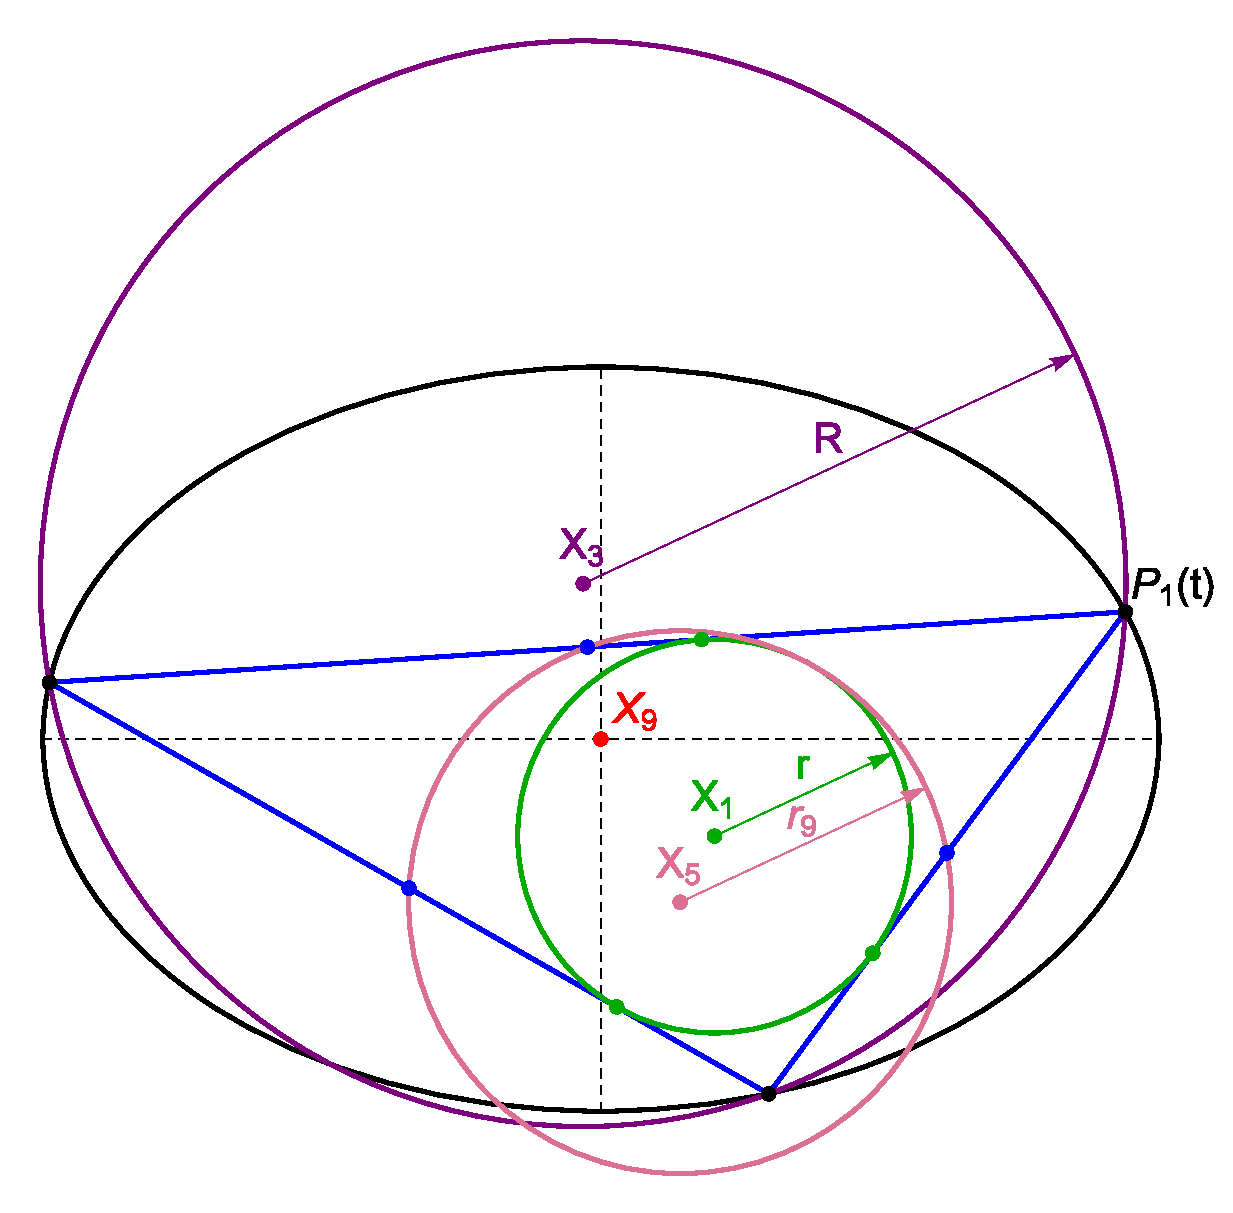
\includegraphics[width=\textwidth]{pics_03_100_radii}
    \caption{The incircle (green), circumcircle (purple), and 9-point (Euler's) circle (pink) of a billiard triangle (blue). These are centered on $X_1$, $X_3$, and $X_5$, respectively. Their radii are the inradius $r$, circumradius $R$, and 9-point circle radius $r_9=2R$. Over the family, the ratio $r/R$ is invariant. In turn this implies an invariant sum of cosines. \href{https://bit.ly/337hvpf}{Live}}
    \label{fig:radii}
\end{figure}

Let $\theta_i$, $r$, $R$, and $A$ denote the ith internal angle, inradius, circumradius, and area of a reference triangle. Primed quantities refer to the excentral triangle. The relations below, appearing in  \cite{johnson1960},  hold for any triangle:

\begin{align}
\sum_{i=1}^{3}{\cos\theta_i}&=1+\frac{r}{R} \label{eqn:03-sum-cos} \\
\prod_{i=1}^{3}{\cos\theta_i'}&=\frac{r}{4R} \label{eqn:03-exc-prod-cos} \\
\frac{A}{A'}&=\frac{r}{2R} \label{eqn:03-area-ratio}
\end{align}

\begin{corollary}
Over billiard 3-periodics, also invariant are the sum of the orbit cosines, the product of excentral cosines, and the ratio of excentral-to-orbit areas.
\label{cor:03-rOvR}
\end{corollary}

Direct calculations yields an expression for the invariant sum of cosines in terms of elliptic billiard constants $J$ and $L$.

\begin{corollary}
$\sum_{i=1}^{3}{\cos\theta_i}=J L - 3$
\end{corollary}

At it will be seen later in \cref{chap:05-billiard}, the above generalizes to $J L -N$ for all $N$.

\section{An interpretation for \torp{$\delta$}{delta}}

The Darboux constant $\delta$ appearing above has a curious geometric interpretation. Recall the power of a point $Q$ with respect to a circle $\Cm=(C_0,R_0)$ is given by $|Q-C_0|^2-R_0^2$, see \cite[Circle Power]{mw}. Let $\Cm$ denote the (moving) circumcircle of billiard 3-periodic, and $O=X_9$ the billiard center.

\begin{proposition}
The power of $O$ with respect to $\Cm$ is constant and equal to $-\delta$.
\label{prop:03-delta}
\end{proposition}

\begin{proof}
Consider an isosceles 3-periodic orbit given by \cref{eq:orbita3-isosceles}.  
	Its circumcircle will be centered at $C_0=[ {\frac { {b}^{2}-\delta}{2b}},0]$ with circumradius $R_0=\frac {{b}^{2}+\delta}{2b}.$
	Therefore, the power of the center of the ellipse with respect to the circumcircle is given by  
	$$|OC_0|^2-R_0^2=\left(\frac { {b}^{2}-\delta}{2b}\right)^2 - \left(\frac {{b}^{2}+\delta}{2b}\right)^2=-\delta.$$
	
	For a generic 3-periodic orbit, the stated invariance is confirmed with a CAS using the vertex parametrization in \cref{prop:03-vtx-param}.  
%	\textcolor{red}{localizar depois}
\end{proof}

\section{Vertex Parametrization with Jacobi's Elliptic Functions}

\subsection{A generic CAP pair}

Consider a general pair of CAP ellipses denoted $\E$ and $\E_c$. We will derive a generic parametrization for the vertices of 3-periodics in such a pair. A first calculation will be helpful. Referring to \cref{fig:ell-ints}(left), the following are coordinates for the intersections $P_2$ and $P_3$ on $\E$ of the two tangents to $\E_c$ seen from a point $P_1=[x_1,y_1]$ also on $\E$:

\begin{figure}
    \centering
    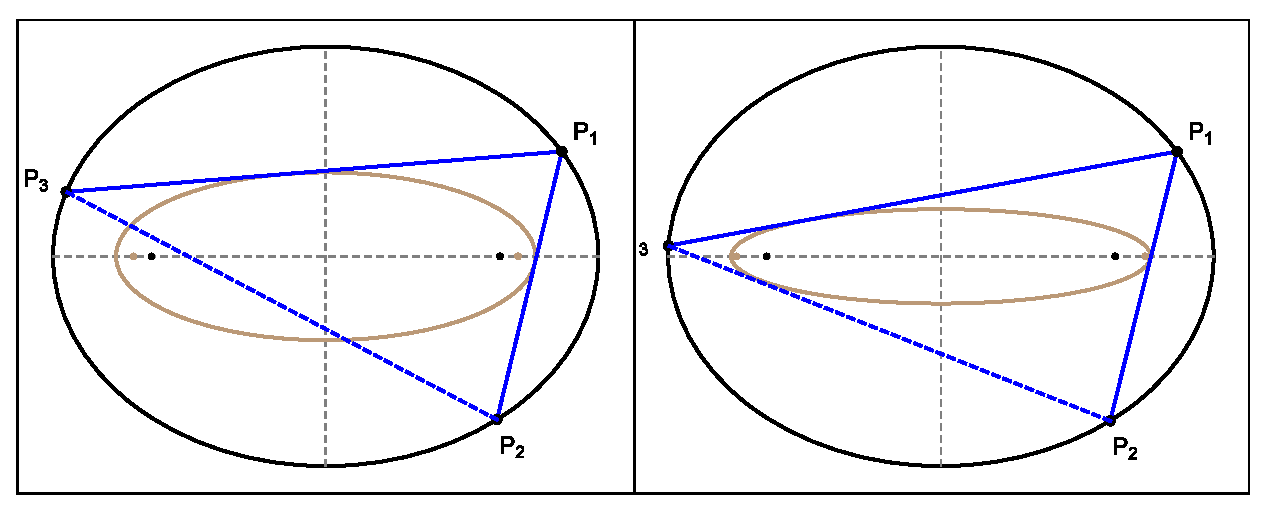
\includegraphics[width=\textwidth]{pics_03_070_ell_ints.eps}
    \caption{\textbf{Left:} Two CAP ellipses (black and brown), and a point $P_1$ on the outer one. The lines thru $P_1$ tangent to the inner ellipse intersect the outer one at $P_2$ and $P_3$. Notice that $P_2 P_3$ cut thru the inner ellipse, i.e., the pair of ellipses does not satisfy Cayley's conditions. \textbf{Right:} the minor axis of the inner ellipse has been scaled such that $P_1 P_2 P_3$ is now a Poncelet triangle.}
    \label{fig:ell-ints}
\end{figure}

\begin{align}
    P_2& =[x_2,y_2]=\frac{1}{k_2}\left[\frac{u_1 x_1 + u_2 y_1}{b} ,  \frac{w_1 x_1 + w_2 y_1}{a} \right] \label{eq:03-n3-conc-general} \\
    P_3&=[x_3,y_3]=\frac{1}{k_2}\left[\frac{w_1 x_1 - w_2 y_1}{b},\frac{w_1 x_1 - w_2 y_1}{a}\right] \nonumber
\end{align}
where:
\begin{align*}
    u_1 &=b\left(a^4  b_c^4 -(a^2 -  a_c^2)^2 b^4 \right) \\
    u_2 &= 2 a k_1 \left( (a^2 + a_c^2)b^2 - b_c^2 a^2\right) \\
    k_1&=\sqrt{ b^2  b_c^2 (a^2 -  a_c^2)  x_1^2 +  a_c^2 a^2(b^2 -  b_c^2)  y_1^2}\\
    k_2 &=\left(\frac{a^2 (b^2 +  b_c^2) - a_c^2 b^2 }{a}x_1\right)^2+ \left(\frac{a^2 (b^2 -  b_c^2) + a_c^2b^2 }{b} y_1\right)^2\\
    w_1&=2 b k_1\left( (b^2 +  b_c^2) a^2 - a_c^2 b^2\right) \\
    w_2&= a\left(a_c^4b^4-a^4(b^2-b_c^2)^2\right)
     %=-a (a^2( b^2 -    b_c^2) -  a_c^2 %b^2) (a^2 (b^2 -   b_c^2) +  a_c^2 b^2)
\end{align*}
 
\subsection{Brocard Porism}

Consider an isosceles Poncelet triangle $\Tm=ABC$ in the Brocard porism, where $AB$ is tangent to $\E$ at one of its minor vertices. Let $|AB|=2d$ and the height be $h$. Let $\zeta=d^2+h^2$. Let the origin $(0,0)$ be at its circumcenter $X_3$. Its vertices will be given by:

\[A=\left[-d ,\frac{d^2-h^2}{2h}\right], \;\;\; B= \left[d,\frac{d^2-h^2}{2h}\right], \;\;\; \left[0 ,\frac{\zeta}{2h}\right] \]


\begin{proposition}\label{prop:pair_brocard}
The Brocard porism containing $\Tm$ as a Poncelet triangle is defined by the following circumcircle $\K_0$ and Brocard inellipse $\E$:

\begin{align*}
\K_0:& x^2+y^2-R^2=0, \;\;\; R=\frac{\zeta}{2h}\\
\E:& -64d^2  h^4  x^2-4  h^2  (9  d^2+h^2)  \zeta  y^2 +4  h  (3  d^2+h^2)  (3  d^2-h^2)  \zeta  y\\&-(d^2-h^2) (9d^2 -h^2) \zeta^2=0
\end{align*}
\end{proposition}

\begin{proof}
The proof follows from $\Tm$, and isosceles Poncelet triangle. Recall that the Brocard inellipse is centered at $X_{39}$. Its perspector is $X_6$, i.e., it will be tangent to $\Tm$ where cevians through $X_6$ intersect it; see \cite[Brocard inellipse]{mw}.
\end{proof}


Consider the pair: circle $x^2+y^2=R^2=(d^2+h^2)^2/(4h^2)$ and   ellipse
$x^2/a^2+(y-y_0)^2/b^2=1$, with  semi-axes
 \[  (a,b)=\left(\frac{d\sqrt{d^2+h^2}}{9d^2+h^2},\frac{4d^2}{9d^2+h^2}\right)
    \]
and center $(0,y_0)$,  $y_0=(9d^4 - h^4)/(2h(9d^2  +  h^3))$.

Vertices $P_i=[x_i,y_i]$, $i=1,2,3$ of Brocard porism triangles are given by:

{\small  
\begin{equation}
    \aligned
    x_1 &= \cos{t}/q_1\\
    y_1 &= \sin{t}/q_1 \\
    x_2 &= -d (d^2 + h^2) ((3 d^2 + h^2)\sin{t} + 2d h \cos{t}- 3 d^2 + h^2)/q_2 \\
    y_2&=-(d^2 + h^2) ((9 d^4 - 2 d^2 h^2 + h^4)\sin{t} - 2 d h (3 d^2 + h^2)\cos{t} - 9 d^4 + h^4)/(2 b q_2) \\
    x_3 &= d (d^2 + h^2) (2 d h \cos{t} - (3 d^2 + h^2) \sin{t} + 3 d^2 - h^2)/q_3\\
    y_3 &=(d^2 + h^2) (2d h (3 d^2 + h^2) \cos{t}+ (9 d^4 - 2 d^2 h^2 + h^4)\sin{t} - 9 d^4 + h^4)/(2 b q_3) \\
    q_1&=(2h)/(d^2+h^2)\\
    q_2&= 2 d h (3 d^2 - h^2)\cos{t} - (9 d^4 - h^4) \sin{t}  + 9 d^4 + 2 d^2 h^2 + h^4\\
    q_3&= 2 d h (3 d^2 - h^2)\cos{t} + (9 d^4 - h^4)\sin{t} - 9 d^4 - 2 d^2 h^2 - h^4
\endaligned
\label{eqn:03-vertices-brocard}
\end{equation}
}



\section{Exercises}

\begin{exercise}
\label{ex:03-circumbilliard} 
Referring to \cref{fig:03-circumbilliard}, show that every triangle has a circumbilliard, i.e., an ellipse to which it is inscribed and to which it is a billiard 3-periodic. Compute the axes of said circumbilliard with respect to triangle vertices. 
\end{exercise}

\begin{figure}
    \centering
    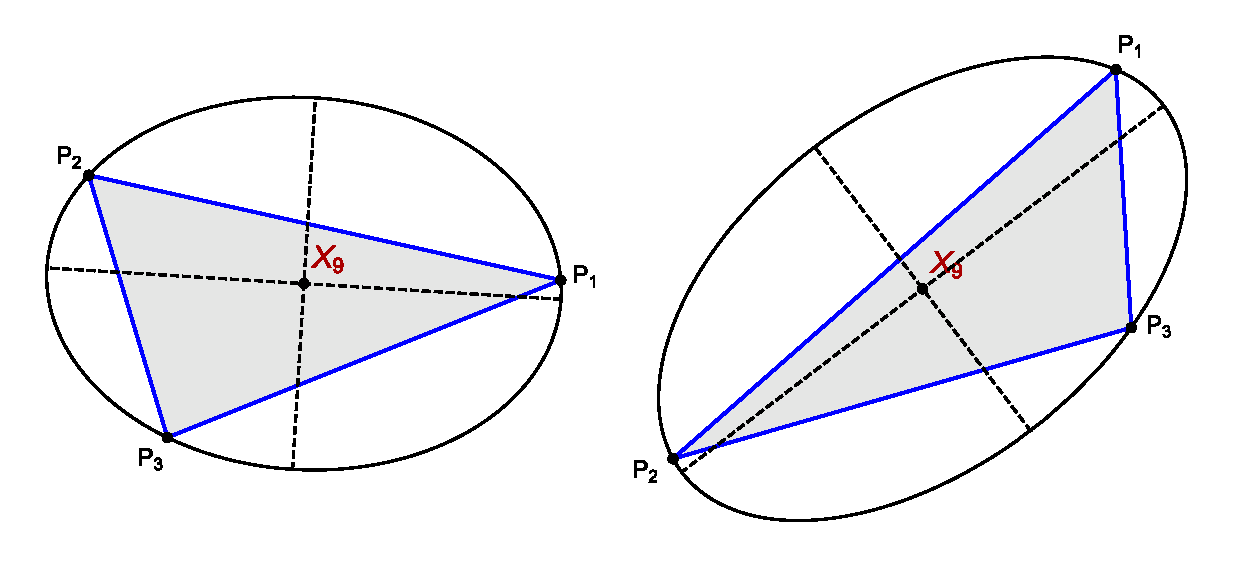
\includegraphics[width=.8\textwidth]{pics_03_320_circumplot.eps}
    \caption{Two random triangles shown with their circumbilliards. \href{https://youtu.be/vSCnorIJ2X8}{Video}}
    \label{fig:03-circumbilliard}
\end{figure}

\begin{exercise}
A pair of circles uniquely defines a {\em pencil} of coaxial circles; see \cite[Limiting Points]{mw}. The pencil contains exactly two circles which degenerate to a point, known as {\em limiting points}. Derive the location of such points for the poristic pair obtained from the image of two confocal ellipses centered at $[0,0]$ and with axes $a,b$ and $a',b'$.
\end{exercise}

\begin{exercise}
Let $\ell_1,\ell_2$ be the limiting points of the two circles which are polar images of a confocal pair $\E,\E'$ with respect to a circle centered on $f_1$. At what aspect ratio $a/b$ of $\E$ will $\ell_2$ coincide with $f_2$?
\end{exercise}

\begin{exercise}
A well-known result is that the inversion of a circle pair $\Cm,\Cm'$ with respect to a circle $\Cm_1$ centered on $\ell_1$ (resp. $\Cm_2$ centered on $\ell_2$) is a pair of concentric circles $\Cm_1'$ and $\Cm_1''$ (resp. $\Cm_1'$ and $\Cm_1''$). Prove the following lesser known result: the ratio of radii between $\Cm_1'$ and $\Cm_1''$ is the same as the ratio between $\Cm_2'$ and $\Cm_2''$. 
\end{exercise}


\begin{figure}
    \centering
    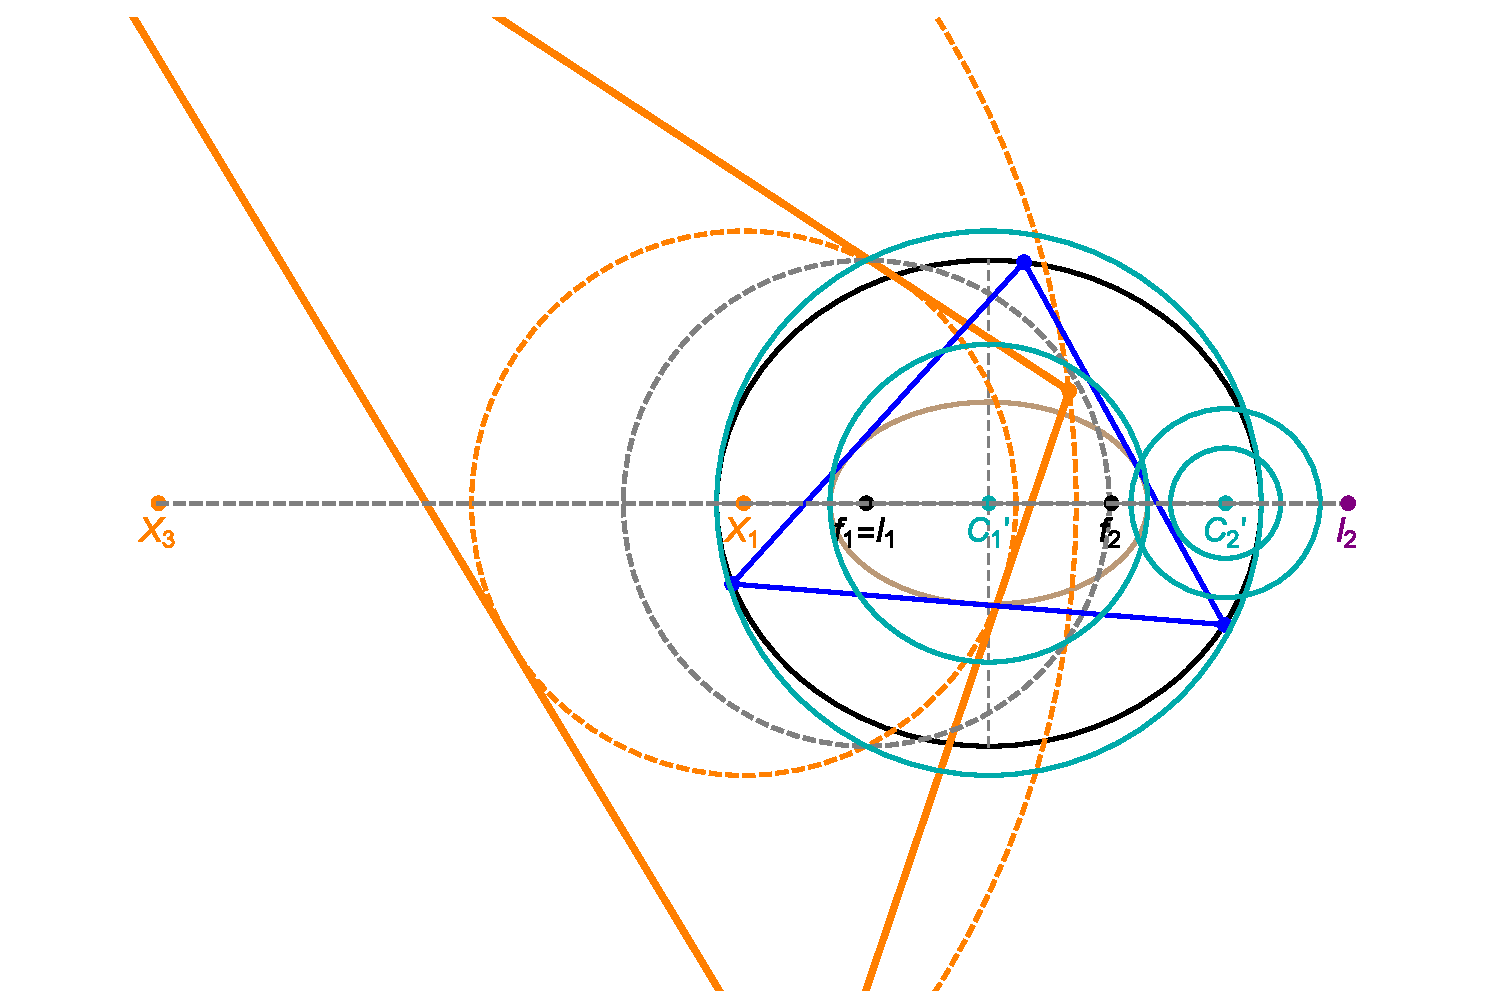
\includegraphics[width=.8\textwidth]{pics_03_210_concentric_inverted_pairs.eps}
    \caption{Concentric circle pairs (light blue) which are the inversions of the circumcircle and incircle (dashed orange) of the bicentric family  (blue) with respect to its two limiting point $\ell_1$ and $\ell_2$. Also shown are Billiard 3-periodics (blue) in the polar pre-image with respect to a circle (dashed gray) -- centered on $f_1=\ell_1$.}
    \label{fig:03-concentric-inverted}
\end{figure}

\begin{exercise}
Referring to \cref{fig:03-concentric-inverted}, let $\Cm,\Cm'$ be the pair of circles which are the polar image of a confocal pair of ellipses $\E,\E'$. Let $\Cm_1', \Cm_1''$ be the inversive images of $\Cm,\Cm'$ wrt to a circle centered on a focus of the ellipse pair. Prove that: (i) $\Cm_1'$ and $\Cm_1''$ are concentric with the ellipse pair and (ii) $\Cm_1'$ (resp. $\Cm_1''$) is externally tangent to $\E$ (resp. $\E'$) at its left and right major vertices.
\end{exercise}


\begin{exercise}
Prove the inversive image of billiard 3-periodics with respect to a focus-centered circle is a non-Ponceletian family inscribed in Pascal's Limaçon whose Gergonne point $X_7$ is stationary; see it \href{https://bit.ly/3edwKD7}{Live}. Indeed, this family has constant perimeter (to be shown later).
\end{exercise}

\begin{exercise}
 Consider the ellipse $x^2/a^2+y^2/b^2=1$. For a  3-periodic  billiard orbit with vertices $P_i=[x_i,y_i]$ (i=1,2,3)  show that:  

\[ 
 \left( x_2\,y_3-x_3\,y_2 \right) x_1\,
y_1+ \left(x_3\,y_1  - x_1\,y_3\right) x_2\, y_2+ \left( x_1\,y_2-x_2\,y_1 \right) x_3
\,y_3=0
\]

\end{exercise}

\begin{exercise} For a  3-periodic  billiard orbit with vertices $P_i=[x_i(t),y_i(t)]$ (i=1,2,3)
Let $C_i(t)=[1/x_i(t),1/y_i(t)]$. 
%Here $P_i(t)=[x_i(t),y_i(t)]$.

Show that the polygon $\{C_1(t),C_2(t),C_3(t)\}$ is a segment that can be bounded or unbounded.
 \label{exe:chap02-inverse-envelope}
\end{exercise}

\begin{exercise} Which simple or self-intersected $N$- gon (closed polygon with $N$ vertices and $N$ sides) can be an orbit on an elliptic billiard? 

 For $N=4$ only the parallelogram can be a non self-intersected orbit on an elliptic billiard, see \cite{connes07}. For the analysis of self-intersected $4-gons$ see \cite{garcia2020-self-intersected}.
\end{exercise}

\section{Research Questions}

\begin{question}
Recall the extouch triangle has vertices at the points of contact of the excircles with a triangle's sidelines \cite[Extouch triangle]{mw}. 
In \cref{chap:04-n3-loci} we show that the vertices of the extouch triangles of billiard 3-periodics coincide with the caustic touchpoints, see it 
\href{https://bit.ly/33PufRv}{Live}. Show that said extouch family is also Ponceletian and concentric with the elliptic billiard; derive expressions for the semi-axes of its elliptic caustic. Is its center a triangle center? 
\label{que:03-extouch}
\end{question}
